\section{Training tips}

\subsection{Activation functions}
Activation functions such as Sigmoid or Tanh saturate
• Gradient is close to 0 or anyway less than 1
• Backpropagation requires gradient multiplications
• Gradient faraway from the output vanishes
• Learning in deep networks does not happen
This is a well-known problem in Recurrent Neural Networks, but it affects also deep networks, and it has always hindered neural network training ...

A possible solution comes by using The ReLU activation function: 
\[g(a)=\text{ReLU}(a=\max(0,a))\]
With a derivative of: 
\[g^\prime(a)=1_{a>0}\]
It has several advantages:
• Faster SGD Convergence (6x w.r.t sigmoid/tanh)
• Sparse activation (only part of hidden units are activated)
• Efficient gradient propagation (no vanishing or exploding gradient problems),
and Efficient computation (just thresholding at zero)
• Scale-invariant: $\max(0,xa)=a\max(0,x)$
\begin{figure}[H]
    \centering
    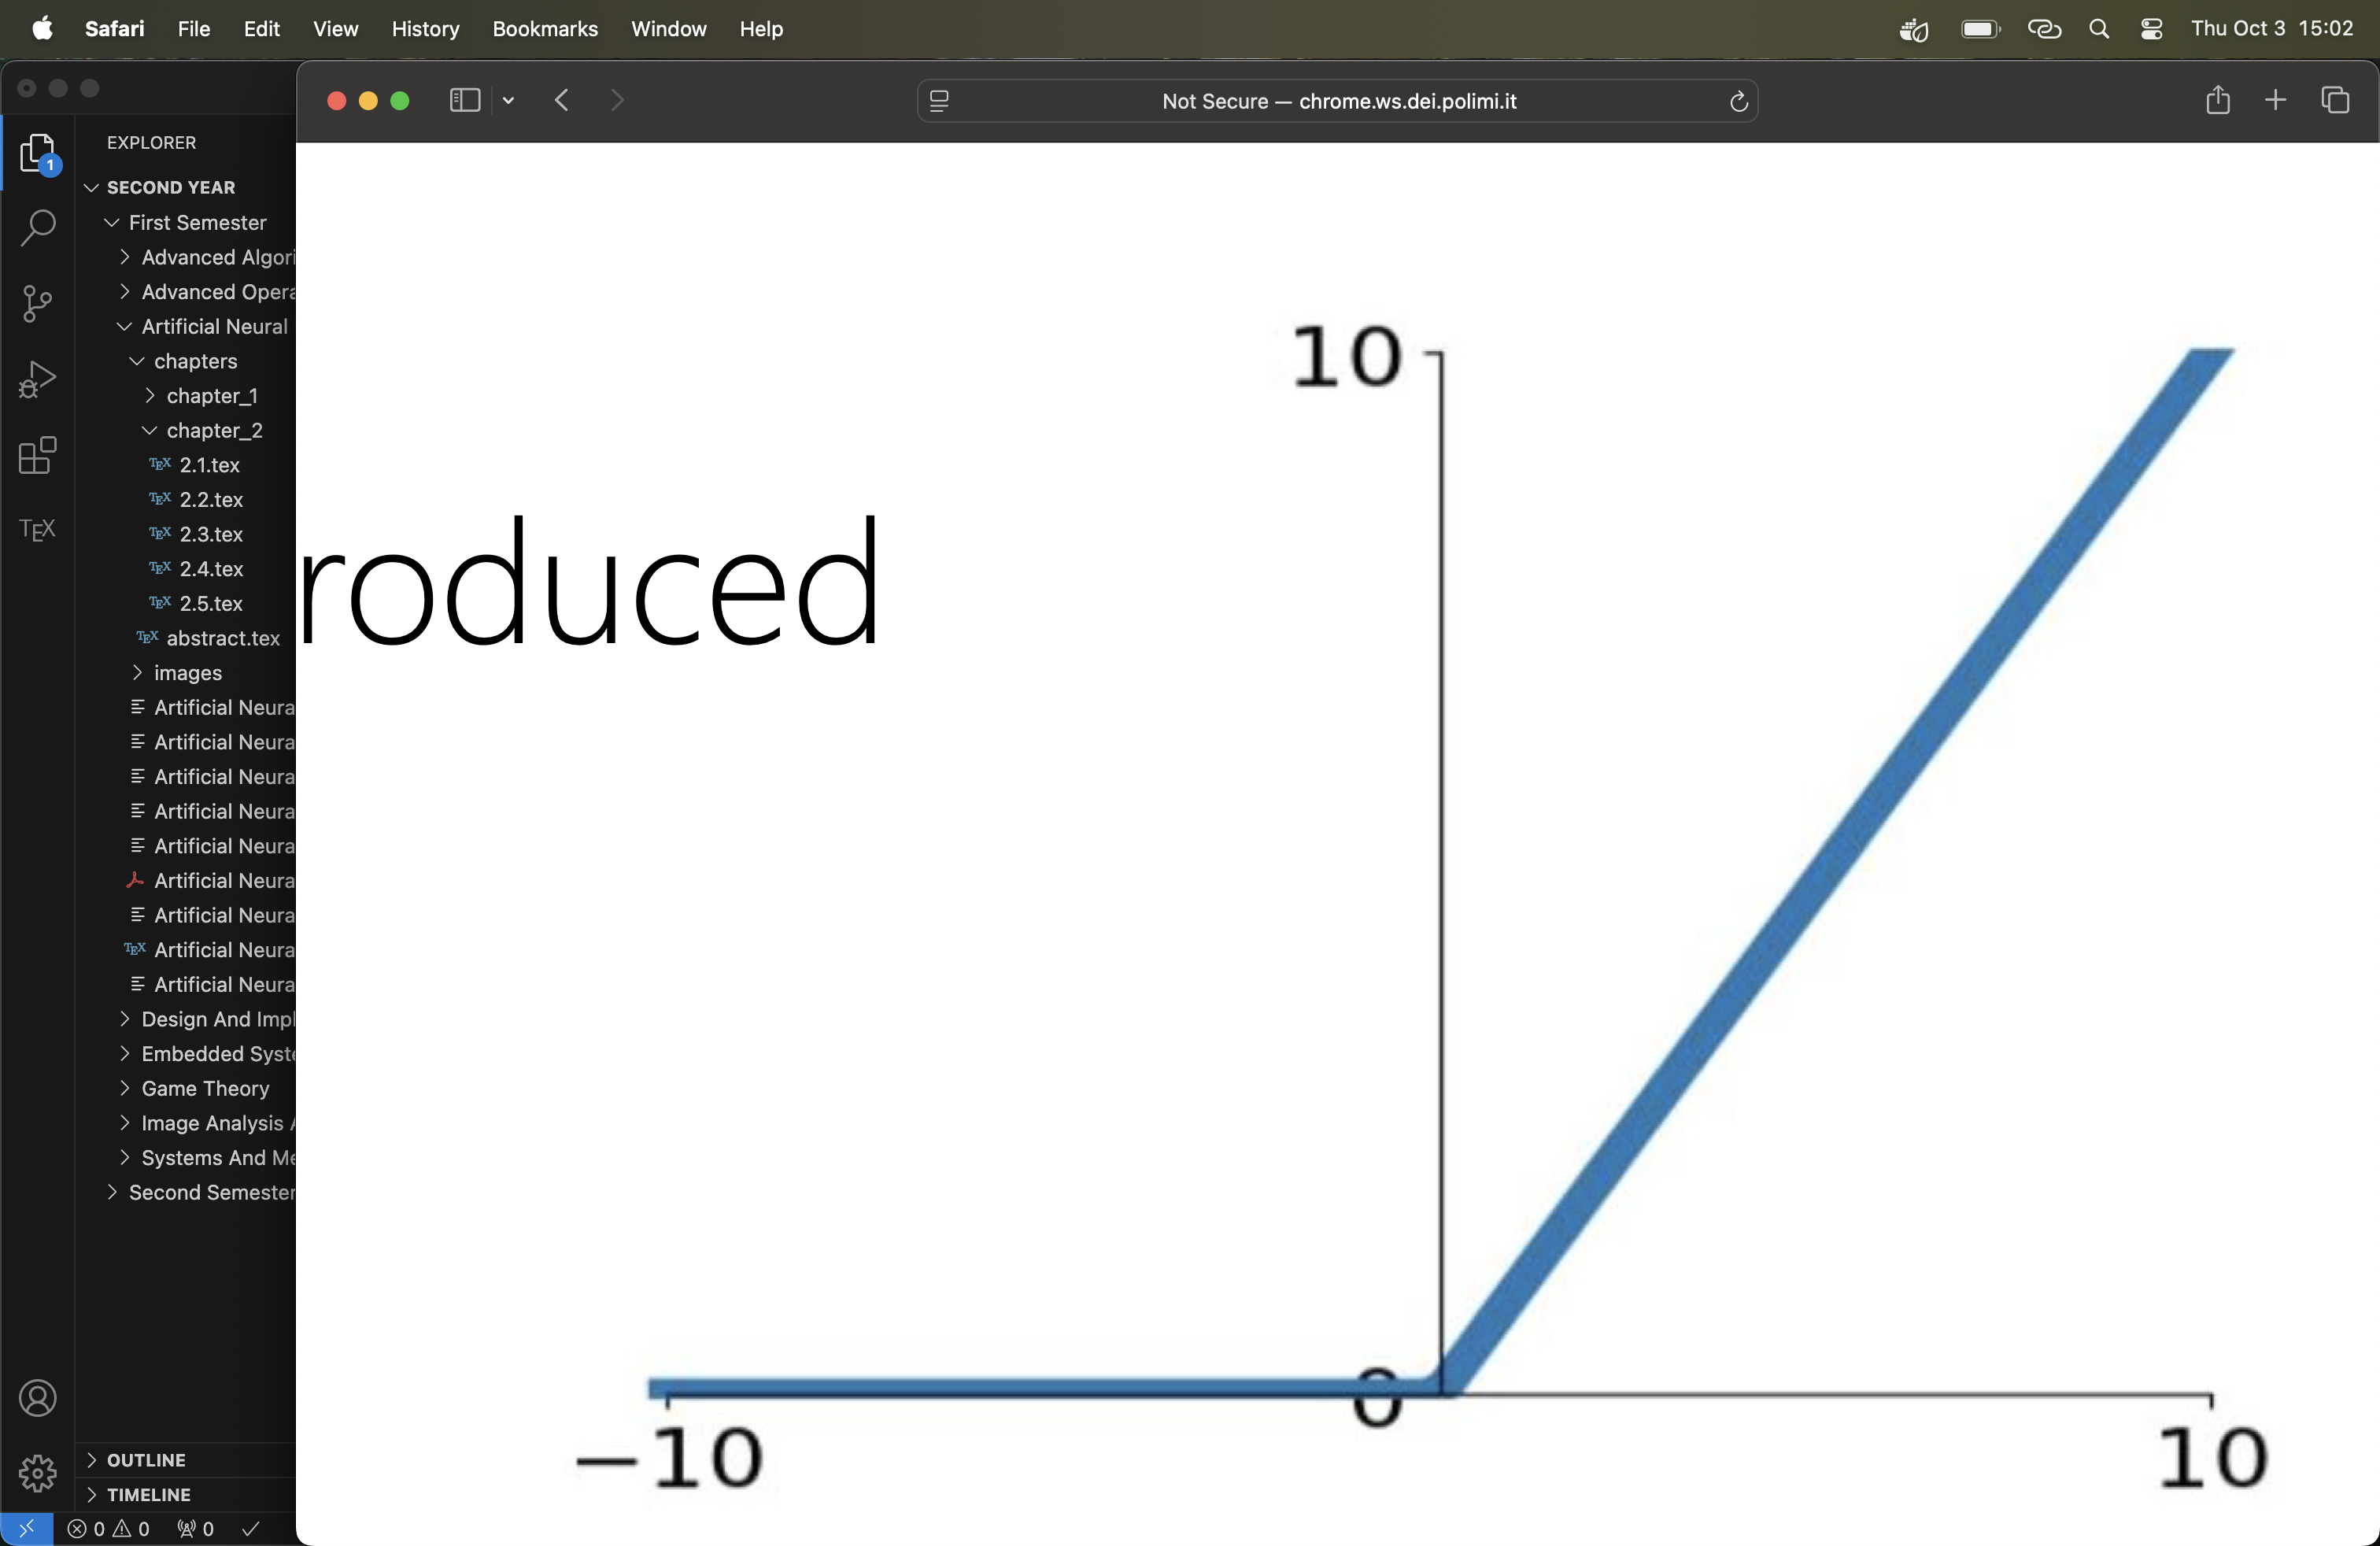
\includegraphics[width=0.75\linewidth]{images/relu.png}
    \caption{Rectified Linear Unit}
\end{figure}
It has potential disadvantages:
• Non-differentiable at zero: however it is differentiable anywhere else
Decreased model
• Non-zero centered output
capacity, it happens with
high learning rates
• Unbounded: Could potentially blow up
• Dying Neurons: ReLU neurons can sometimes be pushed into states in which they become inactive for essentially all inputs. 
  No gradients flow backward through the neuron, and so the neuron becomes stuck and "dies".

Some variants of ReLU are: 
\begin{itemize}
    \item Leaky ReLU: fix for the “dying ReLU” problem: 
        \[f(x)=\begin{cases}
            x \qquad \text{if } x \geq 0 \\
            0.01x \qquad \text{otherwise}
        \end{cases}\]
    \item ELU: try to make the mean activations closer to zero which speeds up learning. 
        Alpha is tuned by hand: 
        \[f(x)=\begin{cases}
            x \qquad \text{if } x \geq 0 \\
            \alpha(e^x-1) \qquad \text{otherwise}
        \end{cases}\]
\end{itemize}

\subsection{Weight initialization}
The final result of gradient descent is affected by weight initialization:
• Zeros: it does not work! All gradient would be zero, no learning will happen
• Big Numbers: bad idea, if unlucky might take very long to converge
• 𝑤 ∼ 𝑁 0, 𝜎2 = 0.01 : good for small networks, but it might be a problem for
deeper neural networks
In deep networks:
• If weights start too small, then gradient shrinks as it passes through each layer
• If the weights in a network start too large, then gradient grows as it passes
through each layer until it’s too massive to be useful
Some proposal to solve this Xavier initialization or He initialization

\paragraph*{Xavier initialization}
Suppose we have an input $\mathbf{x}$ with $I$ components and a linear neuron with random weights $\mathbf{w}$. 
Its output is: 
\[h_j=w_{j,1}x_1+\dots+w_{j,i}x_i+\dots+w_{j,I}x_I\]
We can derive that $w_{j,i}x_i$ is going to have variance: 
\[\text{Var}(w_{j,i}x_i) = \mathbb{E}[x_i]^2\text{Var}(w_{j,i}) + \mathbb{E}[w_{j,i}]^2\text{Var}(x_i) + \text{Var}(w_{j,i})\text{Var}(x_i)\]
Now if our inputs and weights both have mean 0, that simplifies to
\[\text{Var}(w_{j,i}x_i)=\text{Var}(w_{j,i})\text{Var}(x_i)\]
If we assume that $x_i$ and $w_i$ are i.i.d. we obtain: 
\[\text{Var}(h_j)=\text{Var}(w_{j,1}x_1+\dots+w_{j,i}x_i+\dots+w_{j,I}x_I)=I\times\text{Var}(w_i)\text{Var}(x_i)\]
ariance of output is the variance of the input but scaled by $I\times\text{Var}(w_i)$.
If we want the variance of the input and the output to be the same
\[I\times\text{Var}(w_i)=1\]
For this reason Xavier proposes to initialize $w\sim \mathcal{N}\left(0,\frac{1}{n_{\text{in}}}\right)$
Performing similar reasoning for the gradient Glorot and Bengio found: 
\[n_{\text{out}}=\text{Var}(w_j)=1\]
To accommodate for this and Xavier propose $w\sim \mathcal{N}\left(0,\frac{2}{n_{\text{in}}+n_{\text{out}}}\right)$
More recently He proposed, for rectified linear units, $w\sim N\left(0,\frac{2}{n_{\text{in}}}\right)$

\subsection{Adaptive learning}
To avoid local minima can use momentum
\[\mathbf{w}^{k+1}=\mathbf{w}^k-\eta\dfrac{\partial E(\mathbf{w})}{\partial \mathbf{w}}\Bigg|_{\mathbf{w}^k}-\alpha\dfrac{\partial E(\mathbf{w})}{\partial \mathbf{w}}\Bigg|_{\mathbf{w}^{k-1}}\]
Nesterov Accelerated gradient: make a jump as momentum, then adjust
\[\mathbf{w}^{k+\frac{1}{2}}=\mathbf{w}^k-\alpha\dfrac{\partial E(\mathbf{w})}{\partial \mathbf{w}}\Bigg|_{\mathbf{w}^{k-1}}\]
\[\mathbf{w}^{k+1}=\mathbf{w}^k-\eta\dfrac{\partial E(\mathbf{w})}{\partial \mathbf{w}}\Bigg|_{\mathbf{w}^{k+\frac{1}{2}}}\]

Neurons in each layer learn differently
• Gradient magnitudes vary across layers
• Early layers get “vanishing gradients”
• Should ideally use separate adaptive learning rates
Several algorithm proposed:
• Resilient Propagation (Rprop – Riedmiller and Braun 1993)
• Adaptive Gradient (AdaGrad – Duchi et al. 2010)
• RMSprop (SGD + Rprop – Teileman and Hinton 2012)
• AdaDelta (Zeiler et at. 2012)
• Adam (Kingma and Ba, 2012)

\subsection{Batch normalization}
Networks converge faster if inputs have been whitened (zero mean, unit
variances) and are uncorrelated to account for covariate shift.
Networks converge faster if inputs have been whitened (zero mean, unit
variances) and are uncorrelated to account for covariate shift.
We can have internal covariate shift; normalization
could be useful also at the level of hidden layers.
Batch normalization is a technique to cope with this:
• Forces activations to take values on a unit Gaussian
at the beginning of the training
• Adds a BatchNorm layer after fully connected layers
(or convolutional layers), and before nonlinearities.
• Can be interpreted as doing preprocessing at every layer of the network,
but integrated into the network itself in a differentiable way.
In practice
• Each unit’s pre-activation is normalized
(mean subtraction, stddev division)
• During training, mean and stddev are
computed for each minibatch
• Backpropagation takes into account
normalization
• At test time, the global mean / stddev
are used (global statistics are estimated
using training running averages)



\begin{figure}[H]
    \centering
    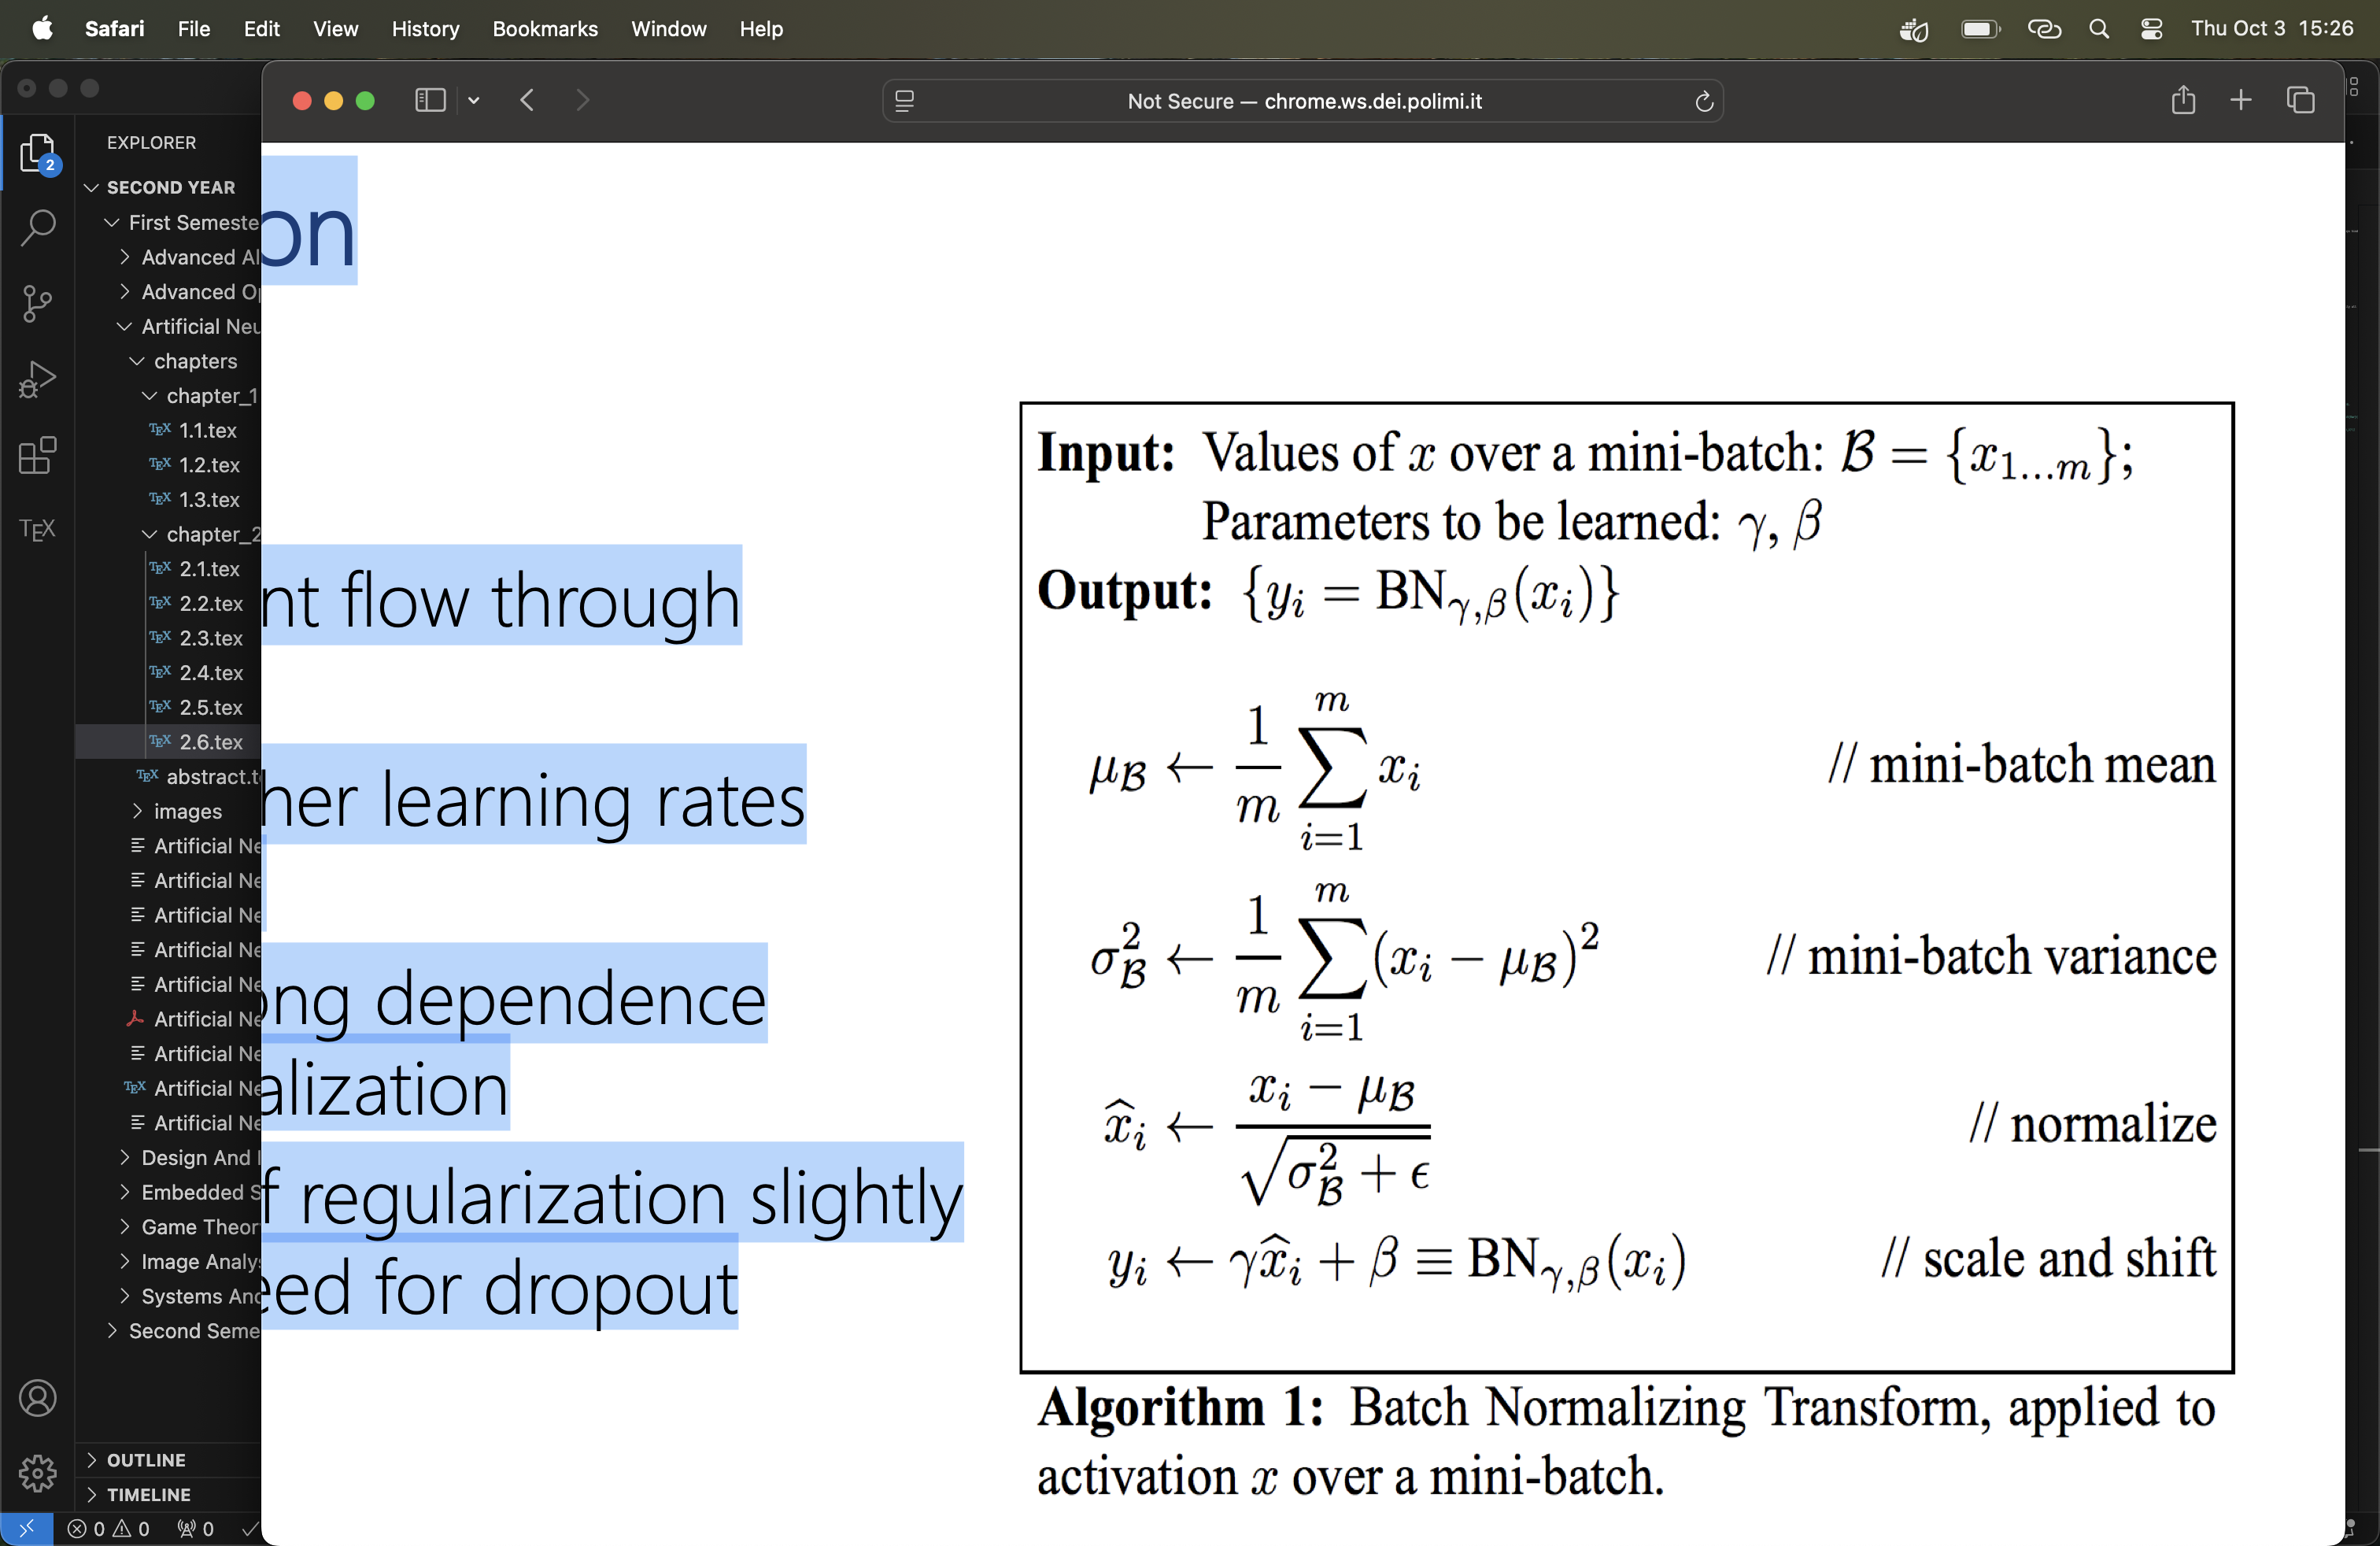
\includegraphics[width=0.75\linewidth]{images/algo.png}
    \caption{Algo}
\end{figure}



Batch Normalization
Has shown to
• Improve gradient flow through
the network
• Allow using higher learning rates
(faster learning)
• Reduce the strong dependence
on weights initialization
• Act as a form of regularization slightly
reducing the need for dropout